\documentclass{standalone}
\usepackage{tikz}
\usepackage{ctex,siunitx}
\usepackage{tkz-euclide}
\usepackage{amsmath}
\usetikzlibrary{patterns, calc}
\usetikzlibrary {decorations.pathmorphing, decorations.pathreplacing, decorations.shapes,}
\begin{document}
\small
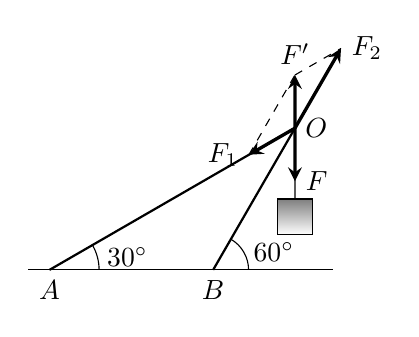
\begin{tikzpicture}[>=stealth,scale=0.9]
  \draw (-0.3,0)--(4,0);
  \draw [ thick](0,0)node[below]{$A$}--(30: 4)node[right]{$O$};
  \draw [ thick](30:4)--(2*1.732-2/1.732,0)node[below]{$B$};
  \draw [very thick, ->] (30:4)--(2*1.732, 2-.75)node[right]{$F$};
  \draw [very thick, ->] (30:4)--(2*1.732, 2+.75)node[above]{$F'$};
  \draw [very thick, ->] (30:4)--(30:4-.75)node[left]{$F_1$};
  \draw [dashed] (30:4-.75)--(2*1.732, 2+.75);
  \draw (.7,0) arc (0:30:.7) node[midway,right]{\ang{30}};
  \draw (2*1.732-2/1.732+.5,0) arc (0:60:.5) node[midway,right]{\ang{60}};
  \draw [very thick, ->] (30:4)--(2*1.732+0.375*1.732, 2+.75*1.5)node[right]{$F_2$};
  \draw [dashed] (2*1.732, 2+.75)--(2*1.732+0.375*1.732, 2+.75*1.5);
  \draw  (30:4)--(2*1.732, 2-1);
  \draw [shade] (2*1.732-.25, 1-.5) rectangle (2*1.732+.25, 1);
\end{tikzpicture}
\end{document}